
%% bare_conf.tex
%% V1.4b
%% 2015/08/26
%% by Michael Shell
%% See:
%% http://www.michaelshell.org/
%% for current contact information.
%%
%% This is a skeleton file demonstrating the use of IEEEtran.cls
%% (requires IEEEtran.cls version 1.8b or later) with an IEEE
%% conference paper.
%%
%% Support sites:
%% http://www.michaelshell.org/tex/ieeetran/
%% http://www.ctan.org/pkg/ieeetran
%% and
%% http://www.ieee.org/

%%*************************************************************************
%% Legal Notice:
%% This code is offered as-is without any warranty either expressed or
%% implied; without even the implied warranty of MERCHANTABILITY or
%% FITNESS FOR A PARTICULAR PURPOSE! 
%% User assumes all risk.
%% In no event shall the IEEE or any contributor to this code be liable for
%% any damages or losses, including, but not limited to, incidental,
%% consequential, or any other damages, resulting from the use or misuse
%% of any information contained here.
%%
%% All comments are the opinions of their respective authors and are not
%% necessarily endorsed by the IEEE.
%%
%% This work is distributed under the LaTeX Project Public License (LPPL)
%% ( http://www.latex-project.org/ ) version 1.3, and may be freely used,
%% distributed and modified. A copy of the LPPL, version 1.3, is included
%% in the base LaTeX documentation of all distributions of LaTeX released
%% 2003/12/01 or later.
%% Retain all contribution notices and credits.
%% ** Modified files should be clearly indicated as such, including  **
%% ** renaming them and changing author support contact information. **
%%*************************************************************************


% *** Authors should verify (and, if needed, correct) their LaTeX system  ***
% *** with the testflow diagnostic prior to trusting their LaTeX platform ***
% *** with production work. The IEEE's font choices and paper sizes can   ***
% *** trigger bugs that do not appear when using other class files.       ***                          ***
% The testflow support page is at:
% http://www.michaelshell.org/tex/testflow/



\documentclass[conference]{IEEEtran}
\usepackage{multirow}
\usepackage{graphicx}
\usepackage{lipsum}  
\usepackage{subfig}
\usepackage{color}
% Some Computer Society conferences also require the compsoc mode option,
% but others use the standard conference format.
%
% If IEEEtran.cls has not been installed into the LaTeX system files,
% manually specify the path to it like:
% \documentclass[conference]{../sty/IEEEtran}





% Some very useful LaTeX packages include:
% (uncomment the ones you want to load)


% *** MISC UTILITY PACKAGES ***
%
%\usepackage{ifpdf}
% Heiko Oberdiek's ifpdf.sty is very useful if you need conditional
% compilation based on whether the output is pdf or dvi.
% usage:
% \ifpdf
%   % pdf code
% \else
%   % dvi code
% \fi
% The latest version of ifpdf.sty can be obtained from:
% http://www.ctan.org/pkg/ifpdf
% Also, note that IEEEtran.cls V1.7 and later provides a builtin
% \ifCLASSINFOpdf conditional that works the same way.
% When switching from latex to pdflatex and vice-versa, the compiler may
% have to be run twice to clear warning/error messages.






% *** CITATION PACKAGES ***
%
%\usepackage{cite}
% cite.sty was written by Donald Arseneau
% V1.6 and later of IEEEtran pre-defines the format of the cite.sty package
% \cite{} output to follow that of the IEEE. Loading the cite package will
% result in citation numbers being automatically sorted and properly
% "compressed/ranged". e.g., [1], [9], [2], [7], [5], [6] without using
% cite.sty will become [1], [2], [5]--[7], [9] using cite.sty. cite.sty's
% \cite will automatically add leading space, if needed. Use cite.sty's
% noadjust option (cite.sty V3.8 and later) if you want to turn this off
% such as if a citation ever needs to be enclosed in parenthesis.
% cite.sty is already installed on most LaTeX systems. Be sure and use
% version 5.0 (2009-03-20) and later if using hyperref.sty.
% The latest version can be obtained at:
% http://www.ctan.org/pkg/cite
% The documentation is contained in the cite.sty file itself.






% *** GRAPHICS RELATED PACKAGES ***
%
\ifCLASSINFOpdf
  %\usepackage[pdftex]{graphicx}
  % declare the path(s) where your graphic files are
  %\graphicspath{{../pdf/}{../jpeg/}}
  % and their extensions so you won't have to specify these with
  % every instance of \includegraphics
  % \DeclareGraphicsExtensions{.pdf,.jpeg,.png}
\else
  % or other class option (dvipsone, dvipdf, if not using dvips). graphicx
  % will default to the driver specified in the system graphics.cfg if no
  % driver is specified.
  % \usepackage[dvips]{graphicx}
  % declare the path(s) where your graphic files are
  % \graphicspath{{../eps/}}
  % and their extensions so you won't have to specify these with
  % every instance of \includegraphics
  % \DeclareGraphicsExtensions{.eps}
\fi
% graphicx was written by David Carlisle and Sebastian Rahtz. It is
% required if you want graphics, photos, etc. graphicx.sty is already
% installed on most LaTeX systems. The latest version and documentation
% can be obtained at: 
% http://www.ctan.org/pkg/graphicx
% Another good source of documentation is "Using Imported Graphics in
% LaTeX2e" by Keith Reckdahl which can be found at:
% http://www.ctan.org/pkg/epslatex
%
% latex, and pdflatex in dvi mode, support graphics in encapsulated
% postscript (.eps) format. pdflatex in pdf mode supports graphics
% in .pdf, .jpeg, .png and .mps (metapost) formats. Users should ensure
% that all non-photo figures use a vector format (.eps, .pdf, .mps) and
% not a bitmapped formats (.jpeg, .png). The IEEE frowns on bitmapped formats
% which can result in "jaggedy"/blurry rendering of lines and letters as
% well as large increases in file sizes.
%
% You can find documentation about the pdfTeX application at:
% http://www.tug.org/applications/pdftex





% *** MATH PACKAGES ***
%
%\usepackage{amsmath}
% A popular package from the American Mathematical Society that provides
% many useful and powerful commands for dealing with mathematics.
%
% Note that the amsmath package sets \interdisplaylinepenalty to 10000
% thus preventing page breaks from occurring within multiline equations. Use:
%\interdisplaylinepenalty=2500
% after loading amsmath to restore such page breaks as IEEEtran.cls normally
% does. amsmath.sty is already installed on most LaTeX systems. The latest
% version and documentation can be obtained at:
% http://www.ctan.org/pkg/amsmath





% *** SPECIALIZED LIST PACKAGES ***
%
%\usepackage{algorithmic}
% algorithmic.sty was written by Peter Williams and Rogerio Brito.
% This package provides an algorithmic environment fo describing algorithms.
% You can use the algorithmic environment in-text or within a figure
% environment to provide for a floating algorithm. Do NOT use the algorithm
% floating environment provided by algorithm.sty (by the same authors) or
% algorithm2e.sty (by Christophe Fiorio) as the IEEE does not use dedicated
% algorithm float types and packages that provide these will not provide
% correct IEEE style captions. The latest version and documentation of
% algorithmic.sty can be obtained at:
% http://www.ctan.org/pkg/algorithms
% Also of interest may be the (relatively newer and more customizable)
% algorithmicx.sty package by Szasz Janos:
% http://www.ctan.org/pkg/algorithmicx




% *** ALIGNMENT PACKAGES ***
%
%\usepackage{array}
% Frank Mittelbach's and David Carlisle's array.sty patches and improves
% the standard LaTeX2e array and tabular environments to provide better
% appearance and additional user controls. As the default LaTeX2e table
% generation code is lacking to the point of almost being broken with
% respect to the quality of the end results, all users are strongly
% advised to use an enhanced (at the very least that provided by array.sty)
% set of table tools. array.sty is already installed on most systems. The
% latest version and documentation can be obtained at:
% http://www.ctan.org/pkg/array


% IEEEtran contains the IEEEeqnarray family of commands that can be used to
% generate multiline equations as well as matrices, tables, etc., of high
% quality.




% *** SUBFIGURE PACKAGES ***
%\ifCLASSOPTIONcompsoc
%  \usepackage[caption=false,font=normalsize,labelfont=sf,textfont=sf]{subfig}
%\else
%  \usepackage[caption=false,font=footnotesize]{subfig}
%\fi
% subfig.sty, written by Steven Douglas Cochran, is the modern replacement
% for subfigure.sty, the latter of which is no longer maintained and is
% incompatible with some LaTeX packages including fixltx2e. However,
% subfig.sty requires and automatically loads Axel Sommerfeldt's caption.sty
% which will override IEEEtran.cls' handling of captions and this will result
% in non-IEEE style figure/table captions. To prevent this problem, be sure
% and invoke subfig.sty's "caption=false" package option (available since
% subfig.sty version 1.3, 2005/06/28) as this is will preserve IEEEtran.cls
% handling of captions.
% Note that the Computer Society format requires a larger sans serif font
% than the serif footnote size font used in traditional IEEE formatting
% and thus the need to invoke different subfig.sty package options depending
% on whether compsoc mode has been enabled.
%
% The latest version and documentation of subfig.sty can be obtained at:
% http://www.ctan.org/pkg/subfig




% *** FLOAT PACKAGES ***
%
%\usepackage{fixltx2e}
% fixltx2e, the successor to the earlier fix2col.sty, was written by
% Frank Mittelbach and David Carlisle. This package corrects a few problems
% in the LaTeX2e kernel, the most notable of which is that in current
% LaTeX2e releases, the ordering of single and double column floats is not
% guaranteed to be preserved. Thus, an unpatched LaTeX2e can allow a
% single column figure to be placed prior to an earlier double column
% figure.
% Be aware that LaTeX2e kernels dated 2015 and later have fixltx2e.sty's
% corrections already built into the system in which case a warning will
% be issued if an attempt is made to load fixltx2e.sty as it is no longer
% needed.
% The latest version and documentation can be found at:
% http://www.ctan.org/pkg/fixltx2e


%\usepackage{stfloats}
% stfloats.sty was written by Sigitas Tolusis. This package gives LaTeX2e
% the ability to do double column floats at the bottom of the page as well
% as the top. (e.g., "\begin{figure*}[!b]" is not normally possible in
% LaTeX2e). It also provides a command:
%\fnbelowfloat
% to enable the placement of footnotes below bottom floats (the standard
% LaTeX2e kernel puts them above bottom floats). This is an invasive package
% which rewrites many portions of the LaTeX2e float routines. It may not work
% with other packages that modify the LaTeX2e float routines. The latest
% version and documentation can be obtained at:
% http://www.ctan.org/pkg/stfloats
% Do not use the stfloats baselinefloat ability as the IEEE does not allow
% \baselineskip to stretch. Authors submitting work to the IEEE should note
% that the IEEE rarely uses double column equations and that authors should try
% to avoid such use. Do not be tempted to use the cuted.sty or midfloat.sty
% packages (also by Sigitas Tolusis) as the IEEE does not format its papers in
% such ways.
% Do not attempt to use stfloats with fixltx2e as they are incompatible.
% Instead, use Morten Hogholm'a dblfloatfix which combines the features
% of both fixltx2e and stfloats:
%
% \usepackage{dblfloatfix}
% The latest version can be found at:
% http://www.ctan.org/pkg/dblfloatfix




% *** PDF, URL AND HYPERLINK PACKAGES ***
%
%\usepackage{url}
% url.sty was written by Donald Arseneau. It provides better support for
% handling and breaking URLs. url.sty is already installed on most LaTeX
% systems. The latest version and documentation can be obtained at:
% http://www.ctan.org/pkg/url
% Basically, \url{my_url_here}.




% *** Do not adjust lengths that control margins, column widths, etc. ***
% *** Do not use packages that alter fonts (such as pslatex).         ***
% There should be no need to do such things with IEEEtran.cls V1.6 and later.
% (Unless specifically asked to do so by the journal or conference you plan
% to submit to, of course. )


% correct bad hyphenation here
\hyphenation{op-tical net-works semi-conduc-tor}


\begin{document}
%
% paper title
% Titles are generally capitalized except for words such as a, an, and, as,
% at, but, by, for, in, nor, of, on, or, the, to and up, which are usually
% not capitalized unless they are the first or last word of the title.
% Linebreaks \\ can be used within to get better formatting as desired.
% Do not put math or special symbols in the title.
\title{Branch Predictor Project}


% author names and affiliations
% use a multiple column layout for up to three different
% affiliations
\author{\IEEEauthorblockN{Danbing Zhu}
\IEEEauthorblockA{Computer Science and Engineering\\
UC San Diego\\
Email: daz054@ucsd.edu}
\and
\IEEEauthorblockA{Kulshreshth Dhiman\\Computer Science and Engineering\\
UC San Diego\\
Email: kdhiman@ucsd.edu}}

% conference papers do not typically use \thanks and this command
% is locked out in conference mode. If really needed, such as for
% the acknowledgment of grants, issue a \IEEEoverridecommandlockouts
% after \documentclass

% for over three affiliations, or if they all won't fit within the width
% of the page, use this alternative format:
% 
%\author{\IEEEauthorblockN{Michael Shell\IEEEauthorrefmark{1},
%Homer Simpson\IEEEauthorrefmark{2},
%James Kirk\IEEEauthorrefmark{3}, 
%Montgomery Scott\IEEEauthorrefmark{3} and
%Eldon Tyrell\IEEEauthorrefmark{4}}
%\IEEEauthorblockA{\IEEEauthorrefmark{1}School of Electrical and Computer Engineering\\
%Georgia Institute of Technology,
%Atlanta, Georgia 30332--0250\\ Email: see http://www.michaelshell.org/contact.html}
%\IEEEauthorblockA{\IEEEauthorrefmark{2}Twentieth Century Fox, Springfield, USA\\
%Email: homer@thesimpsons.com}
%\IEEEauthorblockA{\IEEEauthorrefmark{3}Starfleet Academy, San Francisco, California 96678-2391\\
%Telephone: (800) 555--1212, Fax: (888) 555--1212}
%\IEEEauthorblockA{\IEEEauthorrefmark{4}Tyrell Inc., 123 Replicant Street, Los Angeles, California 90210--4321}}




% use for special paper notices
%\IEEEspecialpapernotice{(Invited Paper)}




% make the title area
\maketitle

% As a general rule, do not put math, special symbols or citations
% in the abstract
\begin{abstract}
		Branch predictor plays a very important role in modern micro-processors especially with depth pipeline. In this report we evaluate the impact of using different storage budgets for 2-level ocal predictor, alpha, Perceptron and G-Share predcitor. 
		Instruction level pipeline is a very important aspect to improve the performance of modern microprocessors. However, the existence of branch instructions causes considerable amount of stalls between instructions and consequently limits the improvement of the throughput of the pipeline. Branch prediction means to make decision for the branches even before their branch conditions are evaluated and thus eliminates the stalls. However, we can see that if the prediction is wrong, the penalty is also huge. So we need to improve the accuracy of the predictors and thus achieve a better performance of the whole pipeline. In this report, we are going to discuss four kinds of predictors. We will evaluate their performance as well as analyze the reasons behind their behaviors.
\end{abstract}

% no keywords




% For peer review papers, you can put extra information on the cover
% page as needed:
% \ifCLASSOPTIONpeerreview
% \begin{center} \bfseries EDICS Category: 3-BBND \end{center}
% \fi
%
% For peerreview papers, this IEEEtran command inserts a page break and
% creates the second title. It will be ignored for other modes.
\IEEEpeerreviewmaketitle



\section{Introduction}
In this project, we use C++ program to simulate the behaviors of four branch predictors. Namely, 2-level local predictor, alpha 21264-like predictor, perceptron predictor and G-share predictor. We evaluate the impact of using different storage budgets for each predictor type, as well as analyzing which (and why) predictors work better for each budget size and trace type. 

\section{Conceptual Description of Predictors}
\subsection{2-Level Local Predictor}
Two level local predictor is based on the idea that miss-rate can be reduced if we take a local history of each branch in consideration. There are two level in this predictor. At the first level, there is Per Branch History Table (PBHT) which has $h$ bit shift registers representing branch results of the most recent $h$ branches.The $h$ bits index into Global Pattern History Table (GPHT) of size $2^{h}$. Each entry in GPHT is a $s$ bits saturating counter which represents branch results of last $h$ branches. The 2-level local predictor takes $a$ least significant bits of each branch address and use them to index PBHT. These $h$ bits index into GPHT provide a saturating counter. We compare this saturating counter to final prediction. We update the contents of history register and saturating counter when the branch is evaluated. Fig \ref{2-level_diagram} illustrates how 2-level local predictor works and Equation (1) shows how to calculate its cost.

    \begin{figure}[!t]
        \centering
        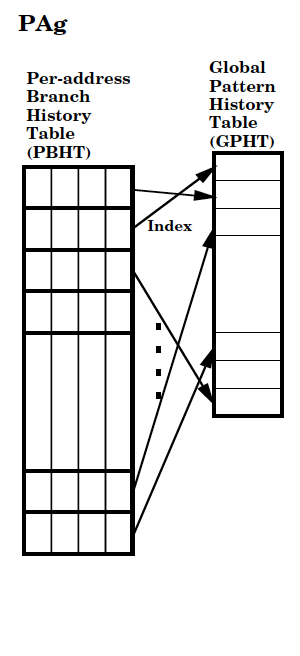
\includegraphics[width=1in]{2-level_diagram}
        \caption{Simulation results for the 2-level local predictor using PAg\cite{twolevel}}
        \label{2-level_diagram}
    \end{figure}
    
    \begin{equation}
    COST = 2^a \cdot h + 2^h \cdot s
    \end{equation}

\subsection{Alpha 21264-like Predictor}
	Some branches are better predicted by local history while some can be better predicted by global history. Alpha 21264-like predictor is a tournament predictor which accounts both local and global history a branch. For the local part, we have 2-level predictor with local history table and local predictor table. For the global part, we have a global predictor. A choice predictor decides which of these predictors (local or global) is best suited for that branch. $a$ least significant bits of program counter index to local history table whose width is $h_l$, and these local histories further index to local predictor table whose width is $s_l$. Global predictor has a table of $s_g$ bits saturating counter index by the $h_g$ bits global history register. The global history register also index to the choice predictor table, where the selected $s_c$ bits saturating counter will decide if we are going to use global or local prediction.Fig \ref{alpha_diagram} illustrates how alpha 21264-like predictor works and Equation (2) shows how to calculate its cost.
\begin{figure}[!t]
        \centering
        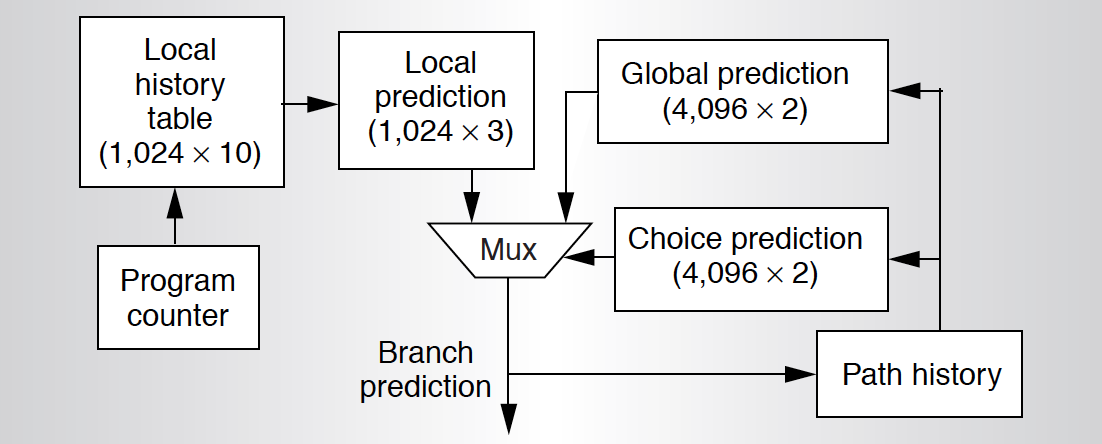
\includegraphics[width=2.3in]{alpha_diagram}
        \caption{Alpha 21264-like predictor\cite{Alpha21264}}
        \label{alpha_diagram}
    \end{figure}
    
    \begin{equation}
    COST = 2^a \cdot h_l + 2^{h_l} \cdot s_l + h_g + 2^{h_g} \cdot s_g + 2^{h_g} \cdot s_c
    \end{equation}
    
\subsection{Perceptron Predictor}
	This predictor utilizes neural methods to predict a branch. Saturating counters in a 2-level predictor are replaced by perceptron. Each perceptron takes the weighted sum of last $h$ branches outcomes. Each weight is s-bit integer and PBHT stores outcomes of most recent $h$ outcomes of a branch. Each perception has $h+1$ weights each $s$ bits. Output function is calculated as follows $$y = w_{0} + \sum_{i=1}^{h} w_{i} * hist_{i}$$
$hist_{i}$ represents is i-th history bit(+1 bit for 0 and -1 for 0 bit). This way perception is able to learn the correlation between a particular branch outcome and current branch behavior. If there is a strong correlation, then weights for that branch outcome increases, and decrease otherwise. We have a table of history register ($h$ bits) indexed by last $a$ bits of the branch address. We have a table of $N$ perceptions, which are indexed by the hash of these $h$ bit history. A simple hash function would be modulo. We update the weights by 1 if history bit and outcome matches and decrease otherwise. This update is done only when there is misprediction or $y$ is less than the threshold(floor($h$*1.93+14)). Equation (3) shows how to calculate the cost of perceptron predictor.

\begin{equation}
    COST = 2^a \cdot h + N \cdot ((1 + h) \cdot s)
    \end{equation}
    
\subsection{G-Share Predictor}
	This prediction scheme is based on the idea that aliasing of branches with same lower address bits and history bits. G-share predictor uses XOR of address and history bits to calculate the index to GPHT. Use of XOR functions improves the utilization of GPHT. If the number of address bits and history bits differs, we take $h$ most significant bits of the address. GPHT entry which is a saturating counter corresponding to XOR outcome will give the final prediction. Fig \ref{gshare_diagram} illustrates how alpha 21264-like predictor works and Equation (2) shows how to calculate its cost.

\begin{figure}[!t]
        \centering
        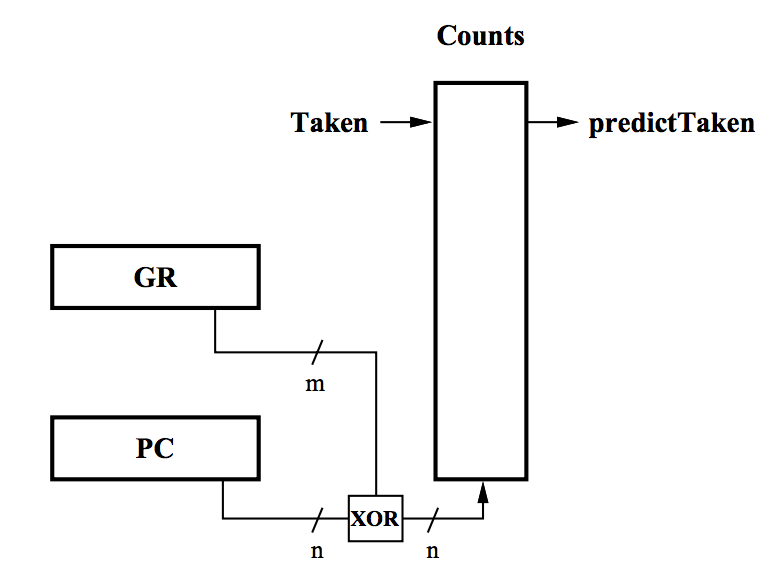
\includegraphics[width=2.3in]{gshare_diagram}
        \caption{G-share predictor\cite{Gshare2}}
        \label{gshare_diagram}
    \end{figure}
    
    \begin{equation}
    COST = h + 2^a \cdot s
    \end{equation}
\section{Simulation Summary}
We will summarize the simulation results of the four predictors with different budget sizes and target trace types in this section.
\subsection{Traces}
We benchmark our predictor for 4 traces namely INT(integer), FP(floating-point), MM(multi-media) and SER(server). In floating programs, branches have spacial locality as they would be part of some for-loop. Also, patterns of these branches are more regular and shorter patterns. We expect that for FP traces, as we increase budget, the number of address bits will have little impact on miss-rate as aliasing is low in FP traces. Also, small but sufficient history bits are sufficient to saturate the miss-rate of FP traces. Branches in integer programs do have spatial locality but not as good as FP. In the case of integer programs branch outcome has more irregularity and data dependence than FP traces.  and thus the branch patterns in integers programs tends to be longer. It requires longer history to efficiently predict the incoming branch. We expect that as the number of history bits increases INT traces would improve miss-rate significantly. Muti-media traces are expected to have high miss-rate as branches are more data-dependent and hence difficult to predict. There is high spatial locality so increasing address bits would have little impact on miss-rate. In the case of MM programs, branches operate on different data each time, for example, pixels in an image. So, a shorter history is preferred for MM as nearby pixels are more correlated that far pixel. We except that MM would work better on shorter history length and number of address bits would have little impact on miss-rate. Server programs execute multiple requests a time. These requests tend to operate in different part of the program. This means that branches in SER would have poor spacial locality. There would an aliasing of branches with same lower LSB bits. Therefore, server trace has a strong correlation between address bits and miss-rate.  In server programs, branches have poor spacial locality due to which branches with same LSB bits will aliase. We expect the server miss-rate to decrease sharply on increasing the number of address bits and number of history bits to have little impact on impact on miss-rate.
\subsection{2-Level Local Predictor}
\subsubsection{Trace Analysis}
We analyze the traces to find the correlation between miss-rate and address and history length. As in Fig \ref{anlys_local_addr} and Fig \ref{anlys_local_hist}, we keep history bits constant, but sufficiently high, and increase the address bits (vice-versa for history). We observe that there is a strong correlation between history bits and INT trace. INT traces requires more history bits, or longer history patterns to better predict the branches. SER traces requires more address bits as budget increases. MM traces doesn't work well on longer history as expect. FP programs require less number of history bits as expected. After 9 bits, there isn't much improvement for MM, INT, FP on increasing address bits and SER, FP on increasing history bits. 
\subsubsection{Results}

%\begin{table}[h]
%\centering
%\begin{tabular}{|l|l|l|l|l|}
%\hline
%Budget & Trace Types &  Miss-rate & Optimal Configuration    & Cost\\ 
%\hline
%\multirow{4}{*}{8K} & DIST-FP-1     &           &\multirow{4}{*}{8K}&  \\ 
%\cline{2-3} \cline{5-5}
%                    & DIST-INT-1    &           &               &    \\ 
%\cline{2-3} \cline{5-5}
%                    & DIST-MM-1     &           &             &    \\
%\cline{2-3} \cline{5-5}
%                    & DIST-SERV-1   &           &              &    \\
%\hline
%\multirow{4}{*}{16K}& DIST-FP-1     &           &\multirow{4}{*}{8K}&  \\ 
%\cline{2-3} \cline{5-5}
%                    & DIST-INT-1    &           &               &    \\ 
%\cline{2-3} \cline{5-5}
%                    & DIST-MM-1     &           &             &    \\
%\cline{2-3} \cline{5-5}
%                    & DIST-SERV-1   &           &              &    \\
%\hline
%\multirow{4}{*}{32K}& DIST-FP-1     &           &\multirow{4}{*}{8K}&  \\ 
%\cline{2-3} \cline{5-5}
%                    & DIST-INT-1    &           &               &    \\ 
%\cline{2-3} \cline{5-5}
%                    & DIST-MM-1     &           &             &    \\
%\cline{2-3} \cline{5-5}
%                    & DIST-SERV-1   &           &              &    \\
%\hline
%\multirow{4}{*}{64K}& DIST-FP-1     &           &\multirow{4}{*}{8K}&  \\ 
%\cline{2-3} \cline{5-5}
%                    & DIST-INT-1    &           &               &    \\ 
%\cline{2-3} \cline{5-5}
%                    & DIST-MM-1     &           &             &    \\
%\cline{2-3} \cline{5-5}
%                    & DIST-SERV-1   &           &              &    \\
%\hline
%\multirow{4}{*}{128K}& DIST-FP-1     &           &\multirow{4}{*}{8K}&  \\ 
%\cline{2-3} \cline{5-5}
%                    & DIST-INT-1    &           &               &    \\ 
%\cline{2-3} \cline{5-5}
%                    & DIST-MM-1     &           &             &    \\
%\cline{2-3} \cline{5-5}
%                    & DIST-SERV-1   &           &              &    \\
%\hline
%\multirow{4}{*}{1M} & DIST-FP-1     &           &\multirow{4}{*}{8K}&  \\ 
%\cline{2-3} \cline{5-5}
%                    & DIST-INT-1    &           &               &    \\ 
%\cline{2-3} \cline{5-5}
%                    & DIST-MM-1     &           &             &    \\
%\cline{2-3} \cline{5-5}
%                    & DIST-SERV-1   &           &              &    \\
%\hline
%\end{tabular}
%\vspace{1mm}
%\caption{Result of 2-level local predictor}
%\label{table1}
%\end{table}

%The raw data is visualized in Fig \ref{fig1}.
\begin{figure}[!t]
\centering
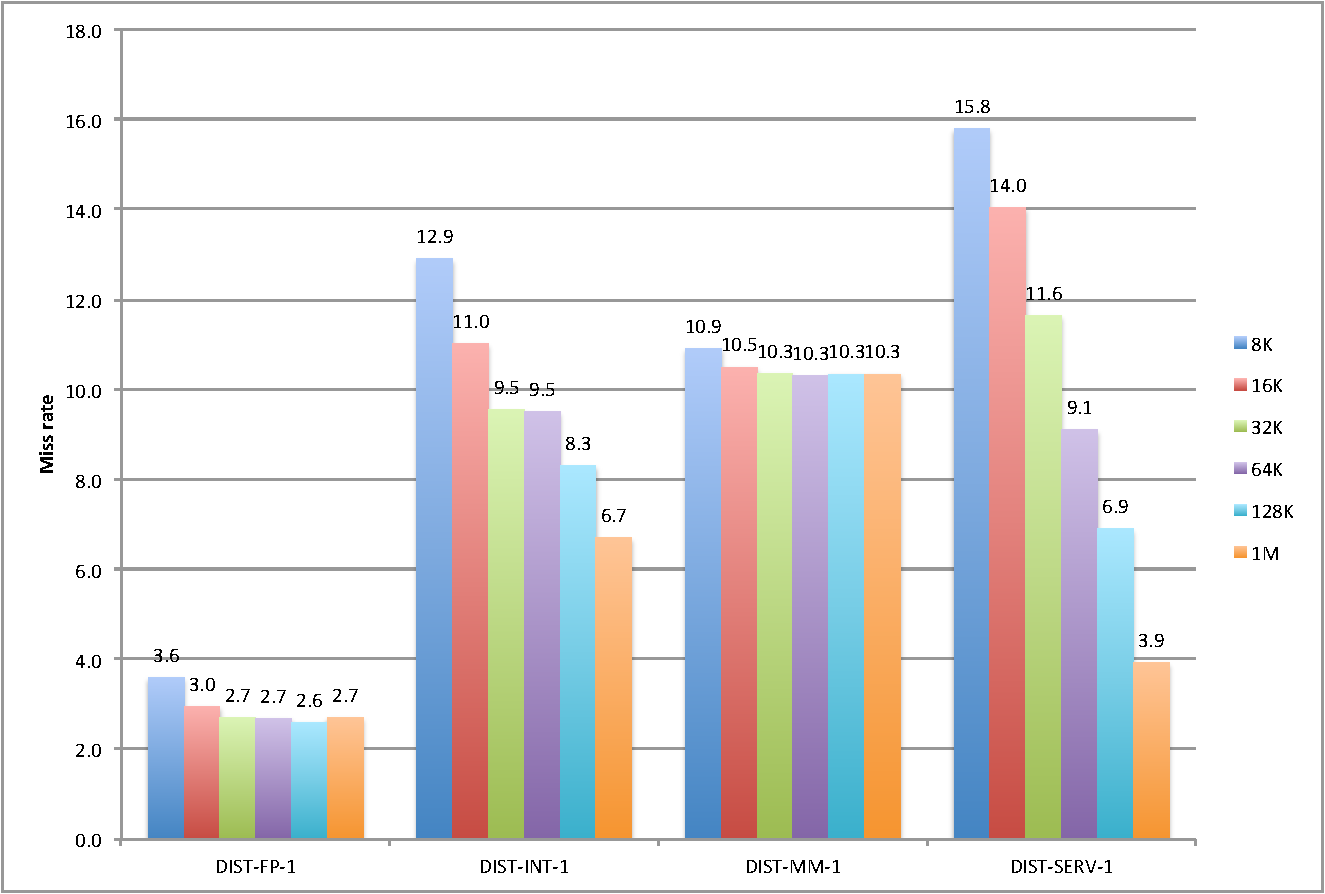
\includegraphics[width=2.3in]{2-level}
\caption{Simulation results for the 2-level local predictor}
\label{fig1}
\end{figure}
We expect that by increasing the address bits we use, the miss rate of the server trace will decrease dramatically due to the reduced aliasing. On the other hand, by increasing the width of the branch history table, we will be able to track branch history better. As a result, we should expect a significant decrease in integer trace's miss rate.  Simulation results for 2-level predictor are shown in Fig \ref{results_local}. 
For INT trace, there is a significant reduction in miss rate mainly due to increase in history bits as budget increase. For SERV, there is a sharp decrease in miss-rate as budget increases. This is mainly due to increase in the number of address bits which reduces branch aliasing. Miss rate is high for multi-media as expected and it doesn't improve significantly as budget increases. Most of the improvement can be incorporated to the reduction in aliasing as address bits increases. FP traces also doesn't improve significantly after 16K budget as history bits are sufficient to capture the branch outcome trends. There is a marginal improvement due to the reduction in aliasing and marginal improvements in branch history lengths. We do notice some small exceptions which are discussed as follows. For integer trace, the miss rate of the predictor doesn't change from 32K budget to 64K budget. After referring to the raw data sheet you will find that the corresponding configurations are 11 bits address and 12 bits history for 32K budget and 12 bits address and 12 bits history for the 64K budget. So this matches our expectation, namely, the number of history bits is the main factor that affects the predictor's performance over integer type trace. On the other hand, you will also notice that the address bits keep increasing as the budget increases. At the same time, the miss rate of the predictor over server trace keeps decreasing sharply, which also matches our expectation.

\begin{figure}[!t]
    \centering
    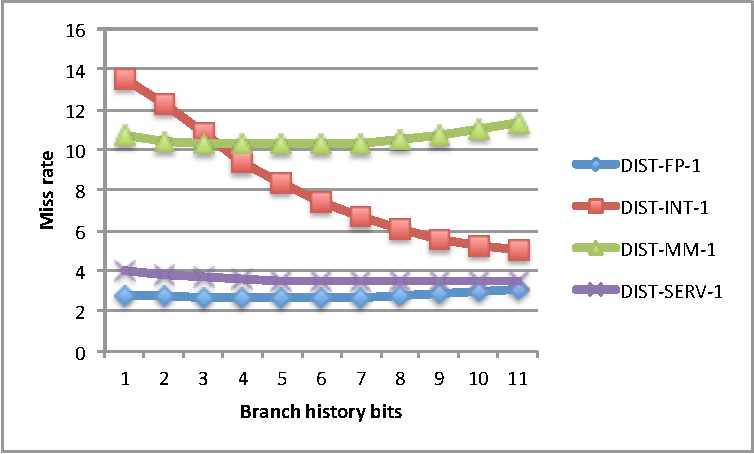
\includegraphics[width=2.3in]{analysis_local_2}
    \caption{Address bits = 2, branch history bits 9 to 19}
    \label{anlys_local_hist}
\end{figure}

\begin{figure}[!t]
    \centering
    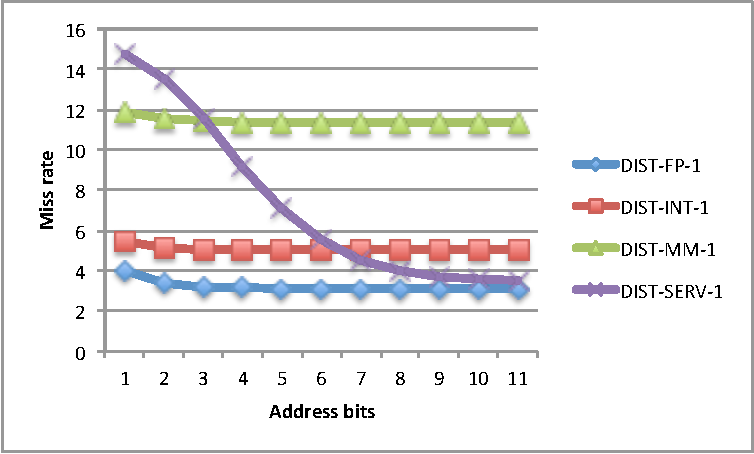
\includegraphics[width=2.3in]{analysis_local_1}
    \caption{Branch history bits = 2, address bits from 9 to 19}
    \label{anlys_local_addr}
\end{figure}


\subsection{Alpha 21264-like Predictor}
\subsubsection{Trace Analysis}
\begin{figure}[!t]
    \centering
    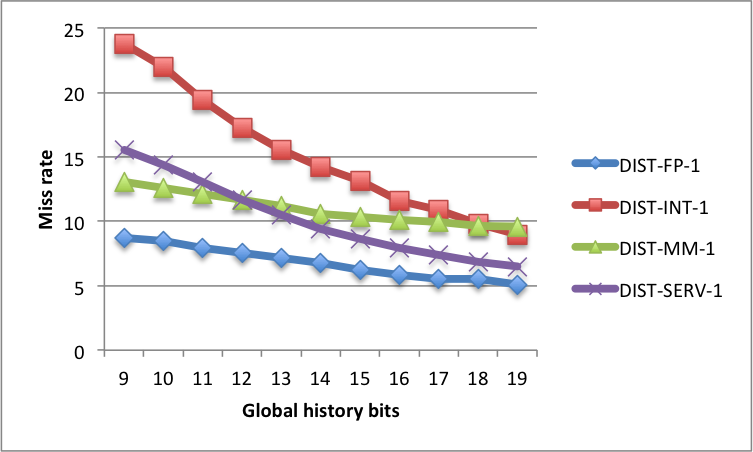
\includegraphics[width=2.3in]{analysis_alpha_ghist.png}
    \caption{Alpha Analysis: Local addr bits = 2, Local hist bits = 2, Global hist bits = 9 to 19}
    \label{anys_alpha_his}
\end{figure}
We have already analyzed 2-level local predictor in the previous section. We analyze the global predictor for different traces. We observe in Fig \ref{anys_alpha_his} that all trace significantly benefits from increasing history bits. Global predictor is able to capture the global trends to branches across all traces. For MM trace miss-rate reduces as history bits are increased. This can be related to exploitation of global patterns of branches. For example, if we are in a particular section of an image, there would be a global pattern among the branches which can be exploited by the global predictor. We observed in the previous section that local branch history doesn't improve MM miss-rate.
\subsubsection{Results}
Simulation results are shown in Fig \ref{results_alpha}. We observe that every trace improves from Alpha prediction scheme. Some trace works better with local prediction while some global. Alpha predictor is able to choose the right balance between local and global predictor. For example, MM traces doesn't work good for local predictor but would work better for global. So, alpha predictor would choose global predictor for MM trace and hence we get significant improvements in miss-rate of MM trace. All results are as expected except few exception. FP trace doesn't improve much as expected. Both global and local predictors saturate as budget increases, so not much improvements. INT and SERV improve sharply as history and address bits increases as budget increases.  
\begin{figure}[!t]
    \centering
    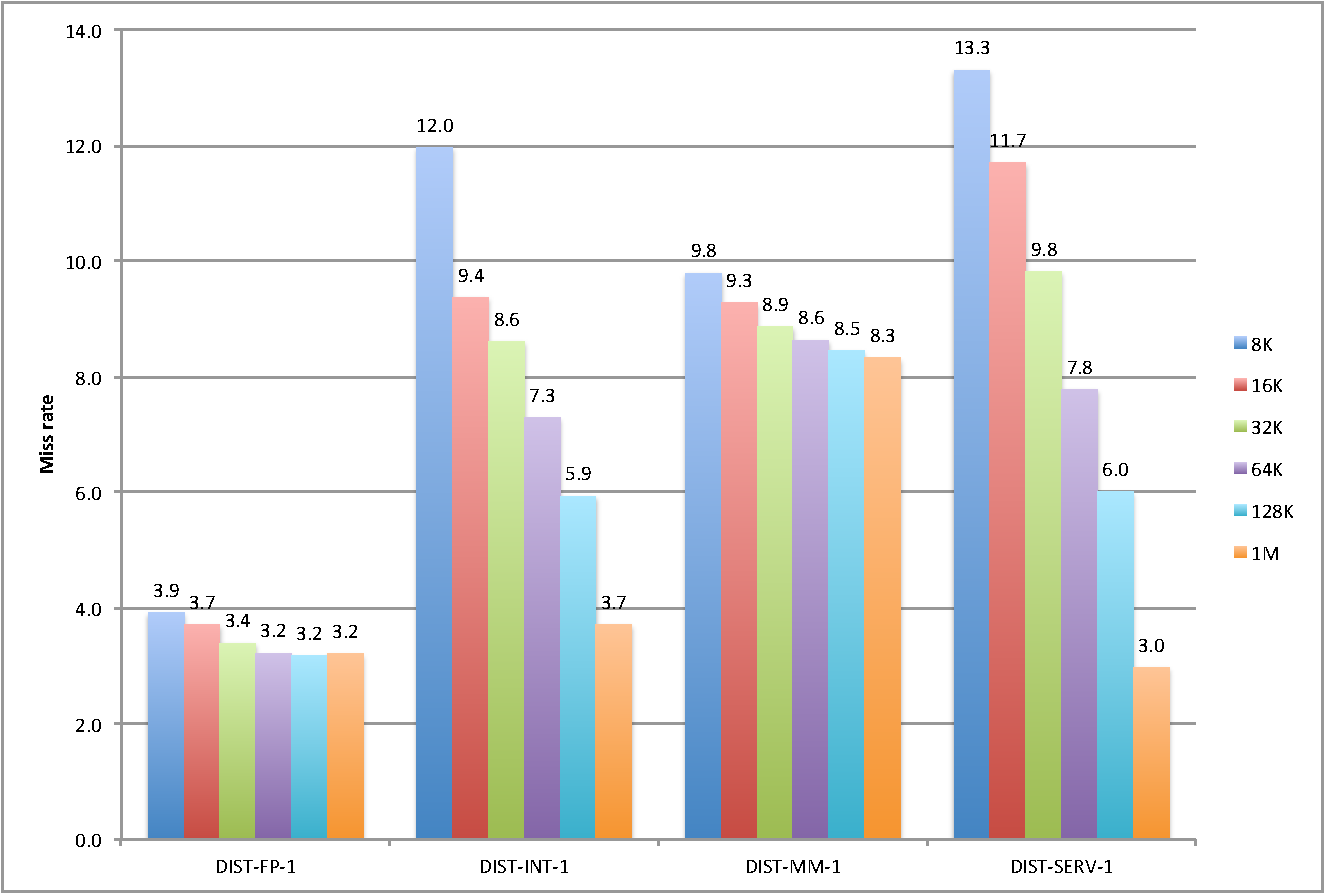
\includegraphics[width=2.3in]{alpha}
    \caption{Simulation results for alpha 21264-like predictor}
    \label{results_alpha}
\end{figure}

\subsubsection{Analysis}

\subsection{Perceptron Predictor}
\subsubsection{Trace Analysis}
\begin{figure}[!t]
    \centering
    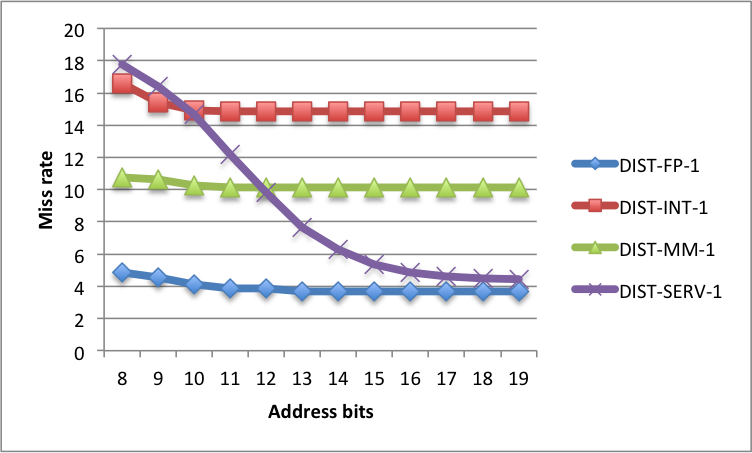
\includegraphics[width=2.3in]{analysis_perceptron_addr.png}
    \caption{Perceptron: Trace analysis for addr bits}
    \label{ana_pep_addr}
\end{figure}
\begin{figure}[!t]
    \centering
    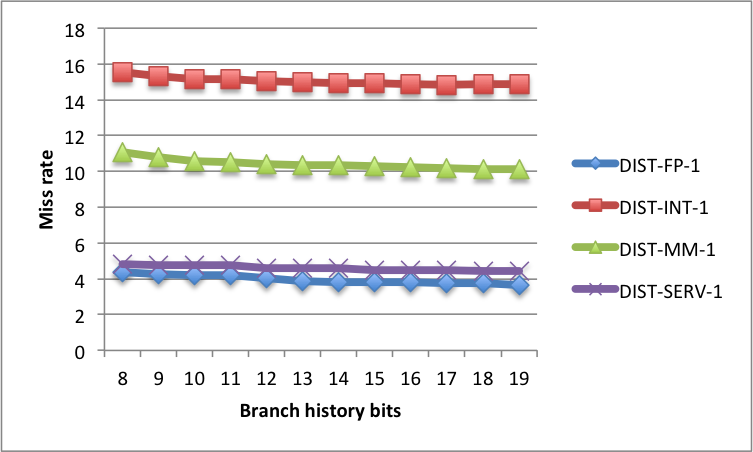
\includegraphics[width=2.3in]{analysis_perceptron_hist.png}
    \caption{Perceptron: Trace analysis for hist bits}
    \label{ana_pep_hist}
\end{figure}
Fig \ref{ana_pep_addr} and Fig \ref{ana_pep_hist} shows the trace analysis for address and history bits respectively. We keep address bits high when analyzing history to rule out any aliasing factor (vice-versa for history bits). We observe that SERV miss-rate decreases sharply due to reduction in aliasing as budget increases. Number of history bits doesn't significanlty improve miss-rate when address bits are high.
\subsubsection{Results}
Simulation results for Perceptron for different budgets are shown in Fig \ref{results_perceptron}.
\begin{figure}[!t]
    \centering
    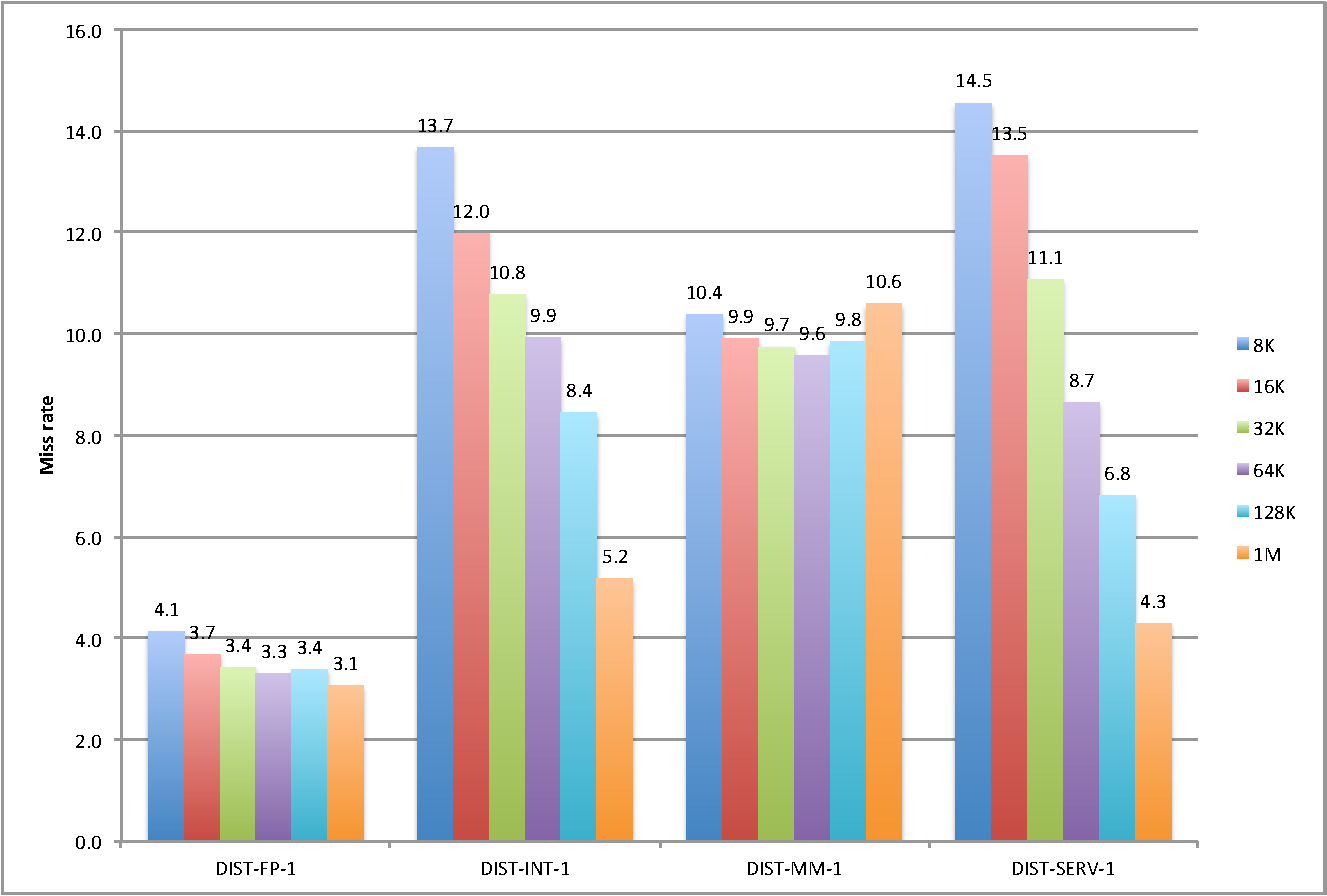
\includegraphics[width=2.3in]{neural}
    \caption{Simulation results for perceptron predictor}
    \label{results_perceptron}
\end{figure}
We observe that INT and SERV traces improves shaply while FP trace also improve significanlty. Expceptinally MM trace miss-rate decreases initially but increases at high budget.
\subsection{G-Share Predictor}
\subsubsection{Trace Analysis}
\begin{figure}[!t]
    \centering
    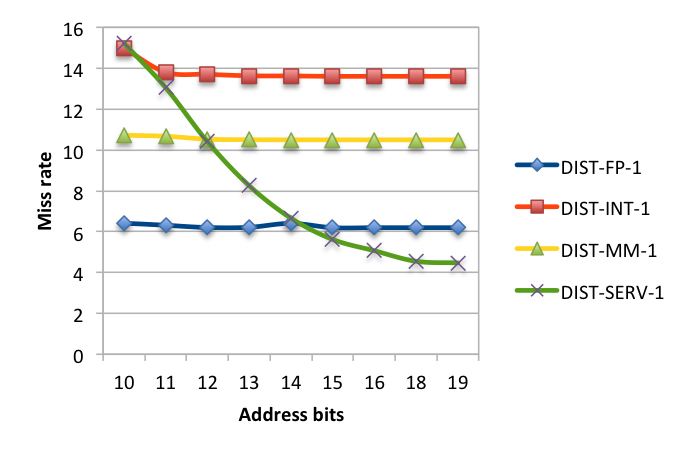
\includegraphics[width=2.3in]{analysis_gshare_addr.png}
    \caption{GShare: Trace analysis for addr bits}
    \label{ana_gshare_addr}
\end{figure}
\begin{figure}[!t]
    \centering
    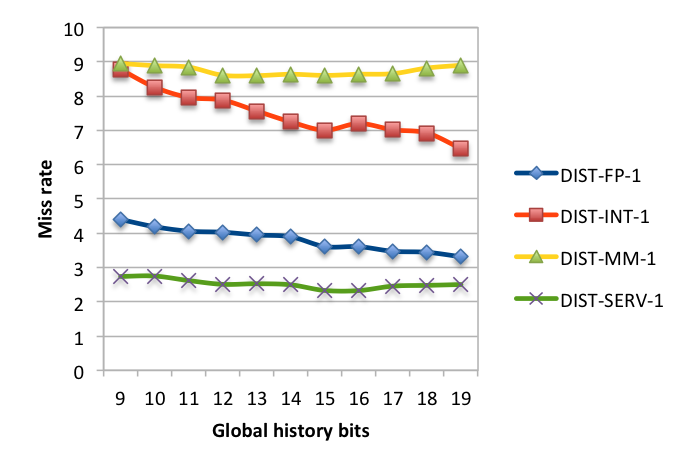
\includegraphics[width=2.3in]{analysis_gshare_hist.png}
    \caption{GShare: Trace analysis for hist bits}
    \label{ana_gshare_hist}
\end{figure}
Fig \ref{ana_gshare_addr} and Fig \ref{ana_gshare_hist} shows the trace analysis for address and history bits respectively. We observe that SERV miss-rate decreases sharply with increasing address bits which is expected. In history analysis figure, we observe that INT trace benefits from increasing history bits which is also expected.
\subsubsection{Results}


\begin{figure}[!t]
    \centering
    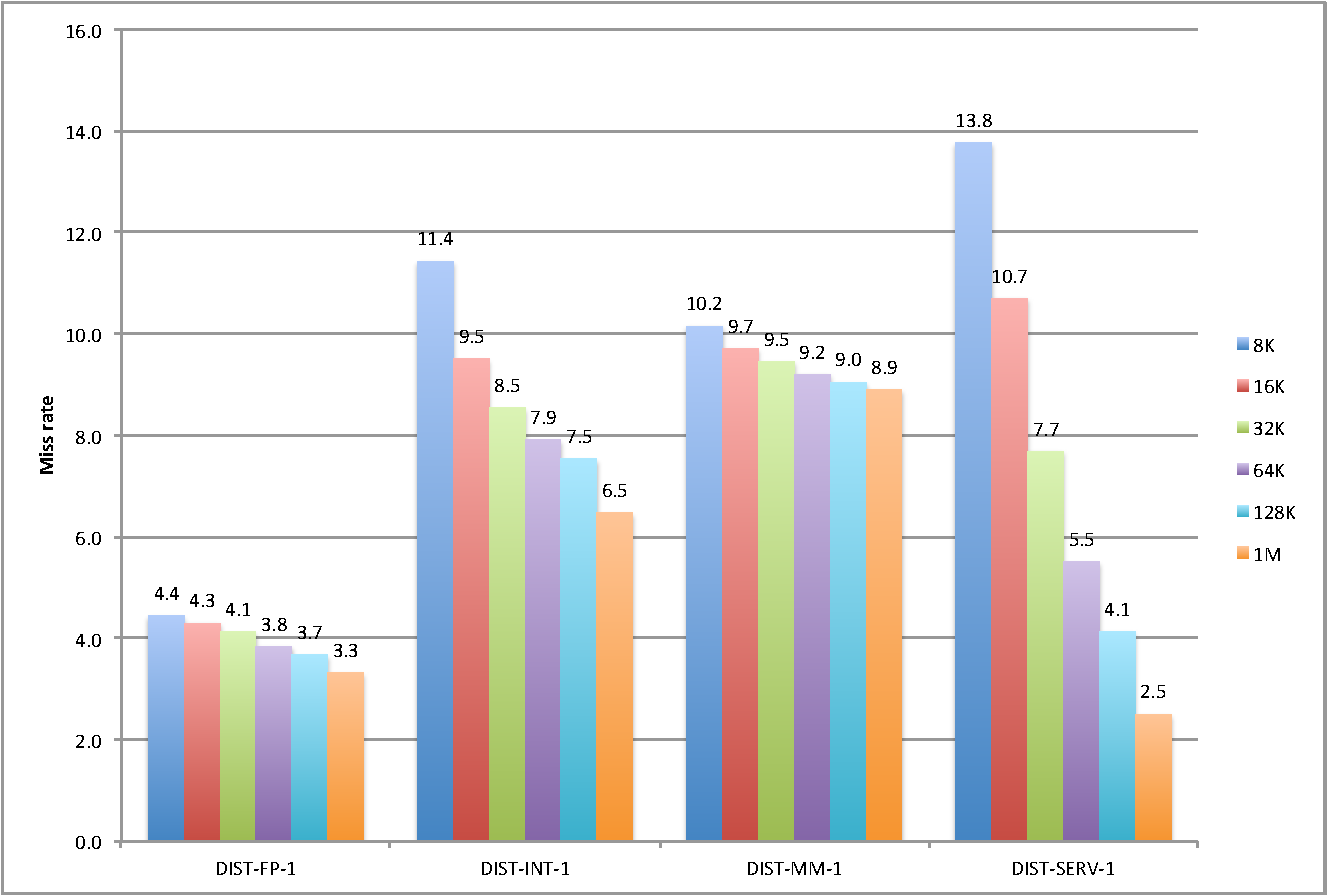
\includegraphics[width=2.3in]{gshare}
    \caption{Simulation results for G-share predictor}
    \label{results_ghsare}
\end{figure}

\subsubsection{Analysis}
Fig \ref{results_ghsare} shows simulation results for GShare. We choose the number of address bits and number of history bits equal for Ghsare simulation. G-share predictor resolves the aliasing problem by XOR the address bits with the global history. So we expect that it should have been the best predictor for server trace type. And we can see from Fig \ref{figa6} that G-share indeed has the best performance over server trace type.
GShare is able to sperate aliasing branches efficiently. Also, traces are benefited from the fact that we are using global history for prediction. As we saw in Trace Analysis of Alpha's global predictor, every trace improved from using global history. GShare adds the benefit of separating aliasing branches. Miss rate for all traces decreases significantly even MM trace. FP and INT traces miss-rate also reduce significantly. 
\begin{figure}[!t]
    \centering
    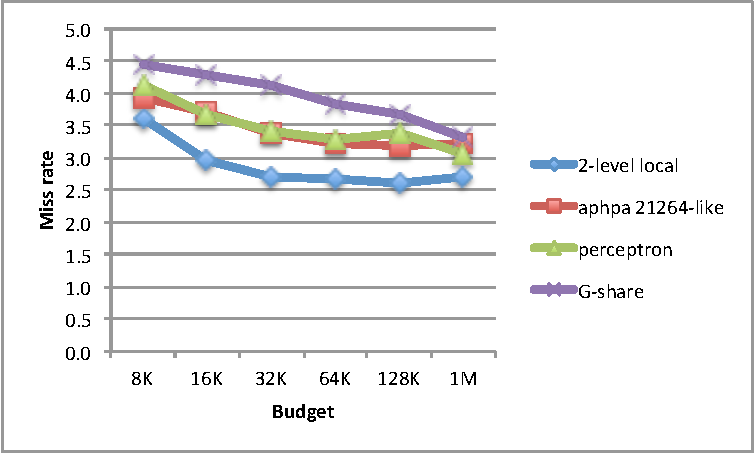
\includegraphics[width=2.3in]{FP}
    \caption{Simulation results for floating point trace type}
    \label{figa3}
\end{figure}

\begin{figure}[!t]
    \centering
    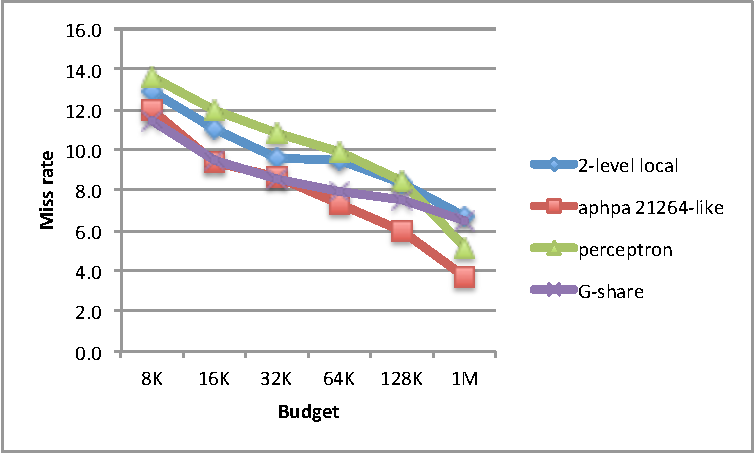
\includegraphics[width=2.3in]{INT}
    \caption{Simulation results for integer trace type}
    \label{figa4}
\end{figure}

\begin{figure}[!t]
    \centering
    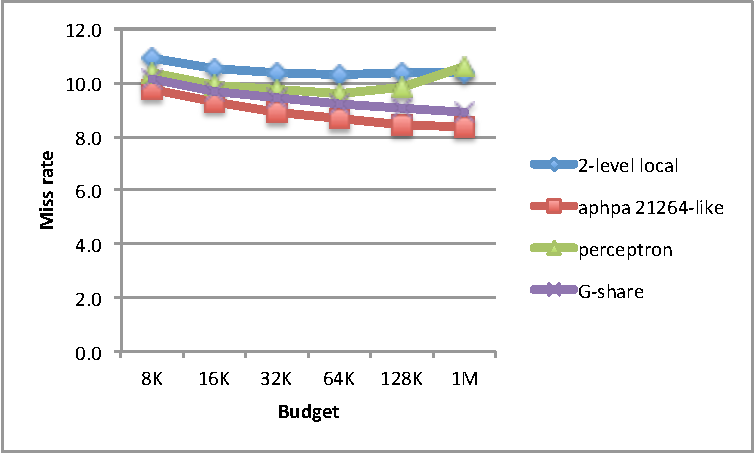
\includegraphics[width=2.3in]{MM}
    \caption{Simulation results for multimedia trace type}
    \label{figa5}
\end{figure}

\begin{figure}[!t]
    \centering
    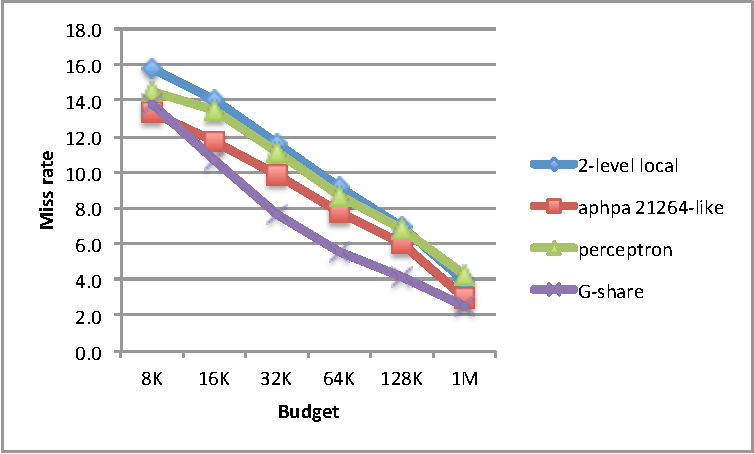
\includegraphics[width=2.3in]{SERVER}
    \caption{Simulation results for server trace type}
    \label{figa6}
\end{figure}


% An example of a floating figure using the graphicx package.
% Note that \label must occur AFTER (or within) \caption.
% For figures, \caption should occur after the \includegraphics.
% Note that IEEEtran v1.7 and later has special internal code that
% is designed to preserve the operation of \label within \caption
% even when the captionsoff option is in effect. However, because
% of issues like this, it may be the safest practice to put all your
% \label just after \caption rather than within \caption{}.
%
% Reminder: the "draftcls" or "draftclsnofoot", not "draft", class
% option should be used if it is desired that the figures are to be
% displayed while in draft mode.
%
%\begin{figure}[!t]
%\centering
%\includegraphics[width=2.4in]{myfigure}
% where an .eps filename suffix will be assumed under latex, 
% and a .pdf suffix will be assumed for pdflatex; or what has been declared
% via \DeclareGraphicsExtensions.
%\caption{Simulation results for the network.}
%\label{fig_sim}
%\end{figure}

% Note that the IEEE typically puts floats only at the top, even when this
% results in a large percentage of a column being occupied by floats.


% An example of a double column floating figure using two subfigures.
% (The subfig.sty package must be loaded for this to work.)
% The subfigure \label commands are set within each subfloat command,
% and the \label for the overall figure must come after \caption.
% \hfil is used as a separator to get equal spacing.
% Watch out that the combined width of all the subfigures on a 
% line do not exceed the text width or a line break will occur.
%
%\begin{figure*}[!t]
%\centering
%\subfloat[Case I]{\includegraphics[width=2.5in]{box}%
%\label{fig_first_case}}
%\hfil
%\subfloat[Case II]{\includegraphics[width=2.5in]{box}%
%\label{fig_second_case}}
%\caption{Simulation results for the network.}
%\label{fig_sim}
%\end{figure*}
%
% Note that often IEEE papers with subfigures do not employ subfigure
% captions (using the optional argument to \subfloat[]), but instead will
% reference/describe all of them (a), (b), etc., within the main caption.
% Be aware that for subfig.sty to generate the (a), (b), etc., subfigure
% labels, the optional argument to \subfloat must be present. If a
% subcaption is not desired, just leave its contents blank,
% e.g., \subfloat[].


% An example of a floating table. Note that, for IEEE style tables, the
% \caption command should come BEFORE the table and, given that table
% captions serve much like titles, are usually capitalized except for words
% such as a, an, and, as, at, but, by, for, in, nor, of, on, or, the, to
% and up, which are usually not capitalized unless they are the first or
% last word of the caption. Table text will default to \footnotesize as
% the IEEE normally uses this smaller font for tables.
% The \label must come after \caption as always.
%
%\begin{table}[!t]
%% increase table row spacing, adjust to taste
%\renewcommand{\arraystretch}{1.3}
% if using array.sty, it might be a good idea to tweak the value of
% \extrarowheight as needed to properly center the text within the cells
%\caption{An Example of a Table}
%\label{table_example}
%\centering
%% Some packages, such as MDW tools, offer better commands for making tables
%% than the plain LaTeX2e tabular which is used here.
%\begin{tabular}{|c||c|}
%\hline
%One & Two\\
%\hline
%Three & Four\\
%\hline
%\end{tabular}
%\end{table}


% Note that the IEEE does not put floats in the very first column
% - or typically anywhere on the first page for that matter. Also,
% in-text middle ("here") positioning is typically not used, but it
% is allowed and encouraged for Computer Society conferences (but
% not Computer Society journals). Most IEEE journals/conferences use
% top floats exclusively. 
% Note that, LaTeX2e, unlike IEEE journals/conferences, places
% footnotes above bottom floats. This can be corrected via the
% \fnbelowfloat command of the stfloats package.




\section{Optimal Predictor}
\subsection{Floating Point}
From Fig \ref{figa3} we can see that 2-level local predictor has the best performance when working with floating point trace. Floating point branches mostly relies on local history of a branch. Two level predictor captures this local branch pattern and hence the best performance for this trace. All other except GShare have high cost than two-level predictor. So, for a given budget, two level can work better than other predictor. Alpha, Neural predictors have parallel graph to two level predictor. 

\subsection{Integer}
For integer trace, G-share predictor and alpha 21264-like predictor have comparable performance at relatively lower budget. But for higher budget, G-share predictor has better performance than others. As we have mentioned before, integer trace have the longest history pattern among all the four traces. And G-share can have the largest number of history bits under the same budget. So that's why G-share predictor has the best performance here, because it can better record the history of the trace.

\subsection{Multimedia}
For multimedia trace, alpha 21264-predictor has the best performance for all budgets. Multimedia trace works best on global predictor. Alpha and GShare uses global history to predict the branch. Alpha performs best on multimedia trace followed by GShare. Alpha has local predictor which adds to global predictor. So, alpha selects the right balance hence works best on this trace.

\subsection{Server}
Finally, for server type trace, G-share predictor perform better than all other predictors. We have discussed in the previous section that for server type trace, the bottleneck that limits its performance is the aliasing problem. And G-share predictor eliminates the aliasing by XOR the address bits with the global history bits. This is the reason behind the observation. At the same time, server type trace can also benefits from G-share predictors' long global history.


\section{Conclusion}
We observe that all predictors' miss-rate decreases as we increase budget. Integer trace works best for predictors with large history length while Server trace requires more address bits to reduce aliasing. Global predictors improves miss-rate of all the traces as predictors are able to exploit global history patterns. Multimedia trace works best on predictor which uses global history. Floating point trace can be improved by exploiting local history a branch. We conclude that in order to have best performance we can choose 2-level predictor for floating point trace, GShare for integer trace, Alpha for multimedia and GShare for server trace. 

% conference papers do not normally have an appendix


% use section* for acknowledgment
%\section*{Acknowledgment}


%The authors would like to thank...





% trigger a \newpage just before the given reference
% number - used to balance the columns on the last page
% adjust value as needed - may need to be readjusted if
% the document is modified later
%\IEEEtriggeratref{8}
% The "triggered" command can be changed if desired:
%\IEEEtriggercmd{\enlargethispage{-5in}}

% references section

% can use a bibliography generated by BibTeX as a .bbl file
% BibTeX documentation can be easily obtained at:
% http://mirror.ctan.org/biblio/bibtex/contrib/doc/
% The IEEEtran BibTeX style support page is at:
% http://www.michaelshell.org/tex/ieeetran/bibtex/
%\bibliographystyle{IEEEtran}
% argument is your BibTeX string definitions and bibliography database(s)
%\bibliography{IEEEabrv,../bib/paper}
%
% <OR> manually copy in the resultant .bbl file
% set second argument of \begin to the number of references
% (used to reserve space for the reference number labels box)
\begin{thebibliography}{1}

\bibitem{IEEEhowto:kopka}
H.~Kopka and P.~W. Daly, \emph{A Guide to \LaTeX}, 3rd~ed.\hskip 1em plus
  0.5em minus 0.4em\relax Harlow, England: Addison-Wesley, 1999.
  
\bibitem{Alpha21264}
Kessler, Richard E. "The alpha 21264 microprocessor." \emph{IEEE micro} 19, no. 2 (1999): 24-36.

\bibitem{bimode}
Lee, Chih-Chieh, I-CK Chen, and Trevor N. Mudge. "The bi-mode branch predictor." In \emph{Microarchitecture, 1997. Proceedings., Thirtieth Annual IEEE/ACM International Symposium on}, pp. 4-13. IEEE, 1997.

\bibitem{twolevel}
Yeh, Tse-Yu, and Yale N. Patt. "Alternative implementations of two-level adaptive branch prediction." In \emph{ACM SIGARCH Computer Architecture News}, vol. 20, no. 2, pp. 124-134. ACM, 1992.

\bibitem{neural}
Jimenez, Daniel A., and Calvin Lin. "Neural methods for dynamic branch prediction." \emph{ACM Transactions on Computer Systems (TOCS)} 20, no. 4 (2002): 369-397.

\bibitem{Gshare1}
McFarling, Scott. \emph{Combining branch predictors}. Vol. 49. Technical Report TN-36, Digital Western Research Laboratory, 1993.

\bibitem{Gshare2}
Daya, Bhavya. "Analysis of Combined Bimodal and GShare Branch Prediction Schemes."

\end{thebibliography}




% that's all folks
\end{document}


